The dynamics of microorganisms are in part the result of microscopic interactions between organisms and their
surrounding environment SOURCE NEEDED. Rather than model this directly, this is typically captured by introducing
stochastic terms to their dynamics. This is done in all the models covered in this report, and for that reason we will give an 
overview of stochastic differential equations (SDEs) followed by their solution via the Monte Carlo methods and the
Fokker-Planck equation.

\subsection{Stochastic Differential Equations and the Fokker-Planck Equation}
For the purposes of this report, SDEs can be conceptually viewed as differential equations
with an additional random term that introduces stochastic fluctuations to their dyamics. 

To illustrate, consider the deterministic differential equation:

\begin{equation*}
    dx = \mu(x(t),t)dt.
\end{equation*}

Here, $x(t)$ is a deterministic variable with a drift term $\mu(x(t), t)$, mapping $\mathbb{R} \times[0, \infty) \to \mathbb{R}$. 
By adding stochasticity through Brownian motion

\begin{equation}\label{eq:sde}
    dX = \mu(X(t),t)dt + \sigma(X(t), t)dW
\end{equation}

where $X(t)$ is now a stochastic process. Here, $\mu(X(t), t)dt$ continues to be the deterministic drift term, while
$\sigma(X_t, t)$ is known as the \textit{diffusion term}, scaling the stochastic fluctuations introduced by the 
Wiener process $W_t$. The increments of $W_t$ are normally distributed as follows:

\begin{equation*}
    dW \sim \mathcal{N}(0, dt).
\end{equation*}

By selecting a sufficiently small time step $\Delta t$, we discretise equation \eqref{eq:sde} to 
numerically approximate the differential as:

\begin{equation}\label{eq:differential_approximation}
    \Delta X = \mu(X(t), t)\Delta t + \sigma(X(t), t) \Delta W
\end{equation}

Equation \eqref{eq:differential_approximation} can be used in an iterative approach to obtain a 
sample trajectory of the SDE in equation \eqref{eq:sde}:

\begin{equation}\label{eq:forward_euler}
    X(t + \Delta t) = X(t) + \Delta X.
\end{equation}

This method is called the Euler-Maruyama method, a stochastic
analogue of the forward Euler method \cite{erban2020stochastic}. 

As $X(t)$ is a stochastic process, 
at any fixed time $t$, $X(t)$ has a distribution described by its 
probability distribution function (PDF).
To obtain the PDF of the random variable $X(t)$ at a given time $t$, two main approaches exist. Firstly, using
the Euler-Maruyama method one can generate
$n$ independent trajectories of the SDE. Provided $n$ is sufficiently large, one can construct 
an empirical density from the realisations of $X(t)$ at time $t$. This approach is called the Monte Carlo method, 
and its accuracy depends on the number of samples $n$. By the central limit theorem, the error in 
estimating the PDF decreases like:

\begin{equation*} 
    \text{Error} \sim \mathcal{O}(n^{-1/2}). 
\end{equation*}


This means that to halve the error we must quadruple the number of samples. This can make Monte Carlo methods
computationally expensive for high precision estimates. 

An alternative approach to determining the PDF is through the Fokker-Planck equation.
The Fokker-Planck equatino is a partial differenial equation (PDE) describing the evolution of the PDF $p(x, t)$ 
associated with $X(t)$. For the SDE given in equation \eqref{eq:sde}, the corresponding Fokker-Planck equation is:

\begin{equation}
    \frac{\partial p(x,t)}{\partial t} = -\frac{\partial}{\partial x}\left[ \mu(x,t) p(x,t) \right] + \frac{1}{2}\frac{\partial^2}{\partial x^2}\left[ \sigma^2(x,t) p(x,t) \right],
\end{equation}

where $p(x,t)$ is the probability density function of the random variable $X_t$. 
Solving this PDE can directly yield the PDF without the sampling noise inherent in Monte Carlo simulations.

For systems involving multiple interacting stochastic processes, we consider a system of coupled SDEs:

\begin{equation}
    d\mathbf{X}_t = \boldsymbol{\mu}(\mathbf{X}_t, t),dt + \boldsymbol{\Sigma}(\mathbf{X}_t, t), d\mathbf{W}_t,
\end{equation}

where $\mathbf{X}_t \in \mathbb{R}^n$ is a vector-valued stochastic process, $\boldsymbol{\mu}(\mathbf{X}_t, t)$ 
is a vector of drift terms, $\boldsymbol{\Sigma}(\mathbf{X}_t, t)$ is a diffusion matrix, and 
$\mathbf{W}_t \in \mathbb{R}^m$ is a vector of independent Wiener processes. The associated Fokker-Planck
equation describing the evolution of the joint probability density $p(\mathbf{x}, t)$ for the system is given by:

\begin{equation}
    \frac{\partial p(\mathbf{x}, t)}{\partial t} = -\nabla_{\mathbf{x}} \cdot \left[ \boldsymbol{\mu}(\mathbf{x}, t) p(\mathbf{x}, t) \right] 
    + \frac{1}{2} \nabla_{\mathbf{x}} \cdot \left( \nabla_{\mathbf{x}} \cdot \left[ \boldsymbol{\Sigma}(\mathbf{x}, t) \boldsymbol{\Sigma}(\mathbf{x}, t)^T p(\mathbf{x}, t) \right] \right).
\end{equation}

where $\nabla_{\mathbf{x}}$ is the gradient operator with respect to the spatial variables $\mathbf{x}$.
Solving this PDE provides a direct method for obtaining the joint probability distributions of systems of 
interacting stochastic systems.

\subsection{Model 1: Pure Stochastic Model}\label{sec:pure_stoch_model}
The first model we present considers an elliptic cell with orientation $\theta$ placed within a
channel of infinite width and fixed height $H$. The setup for this model is illustrated
in Figure \ref{fig:model1_setup}.

\begin{figure}[htbp]
    \centering
    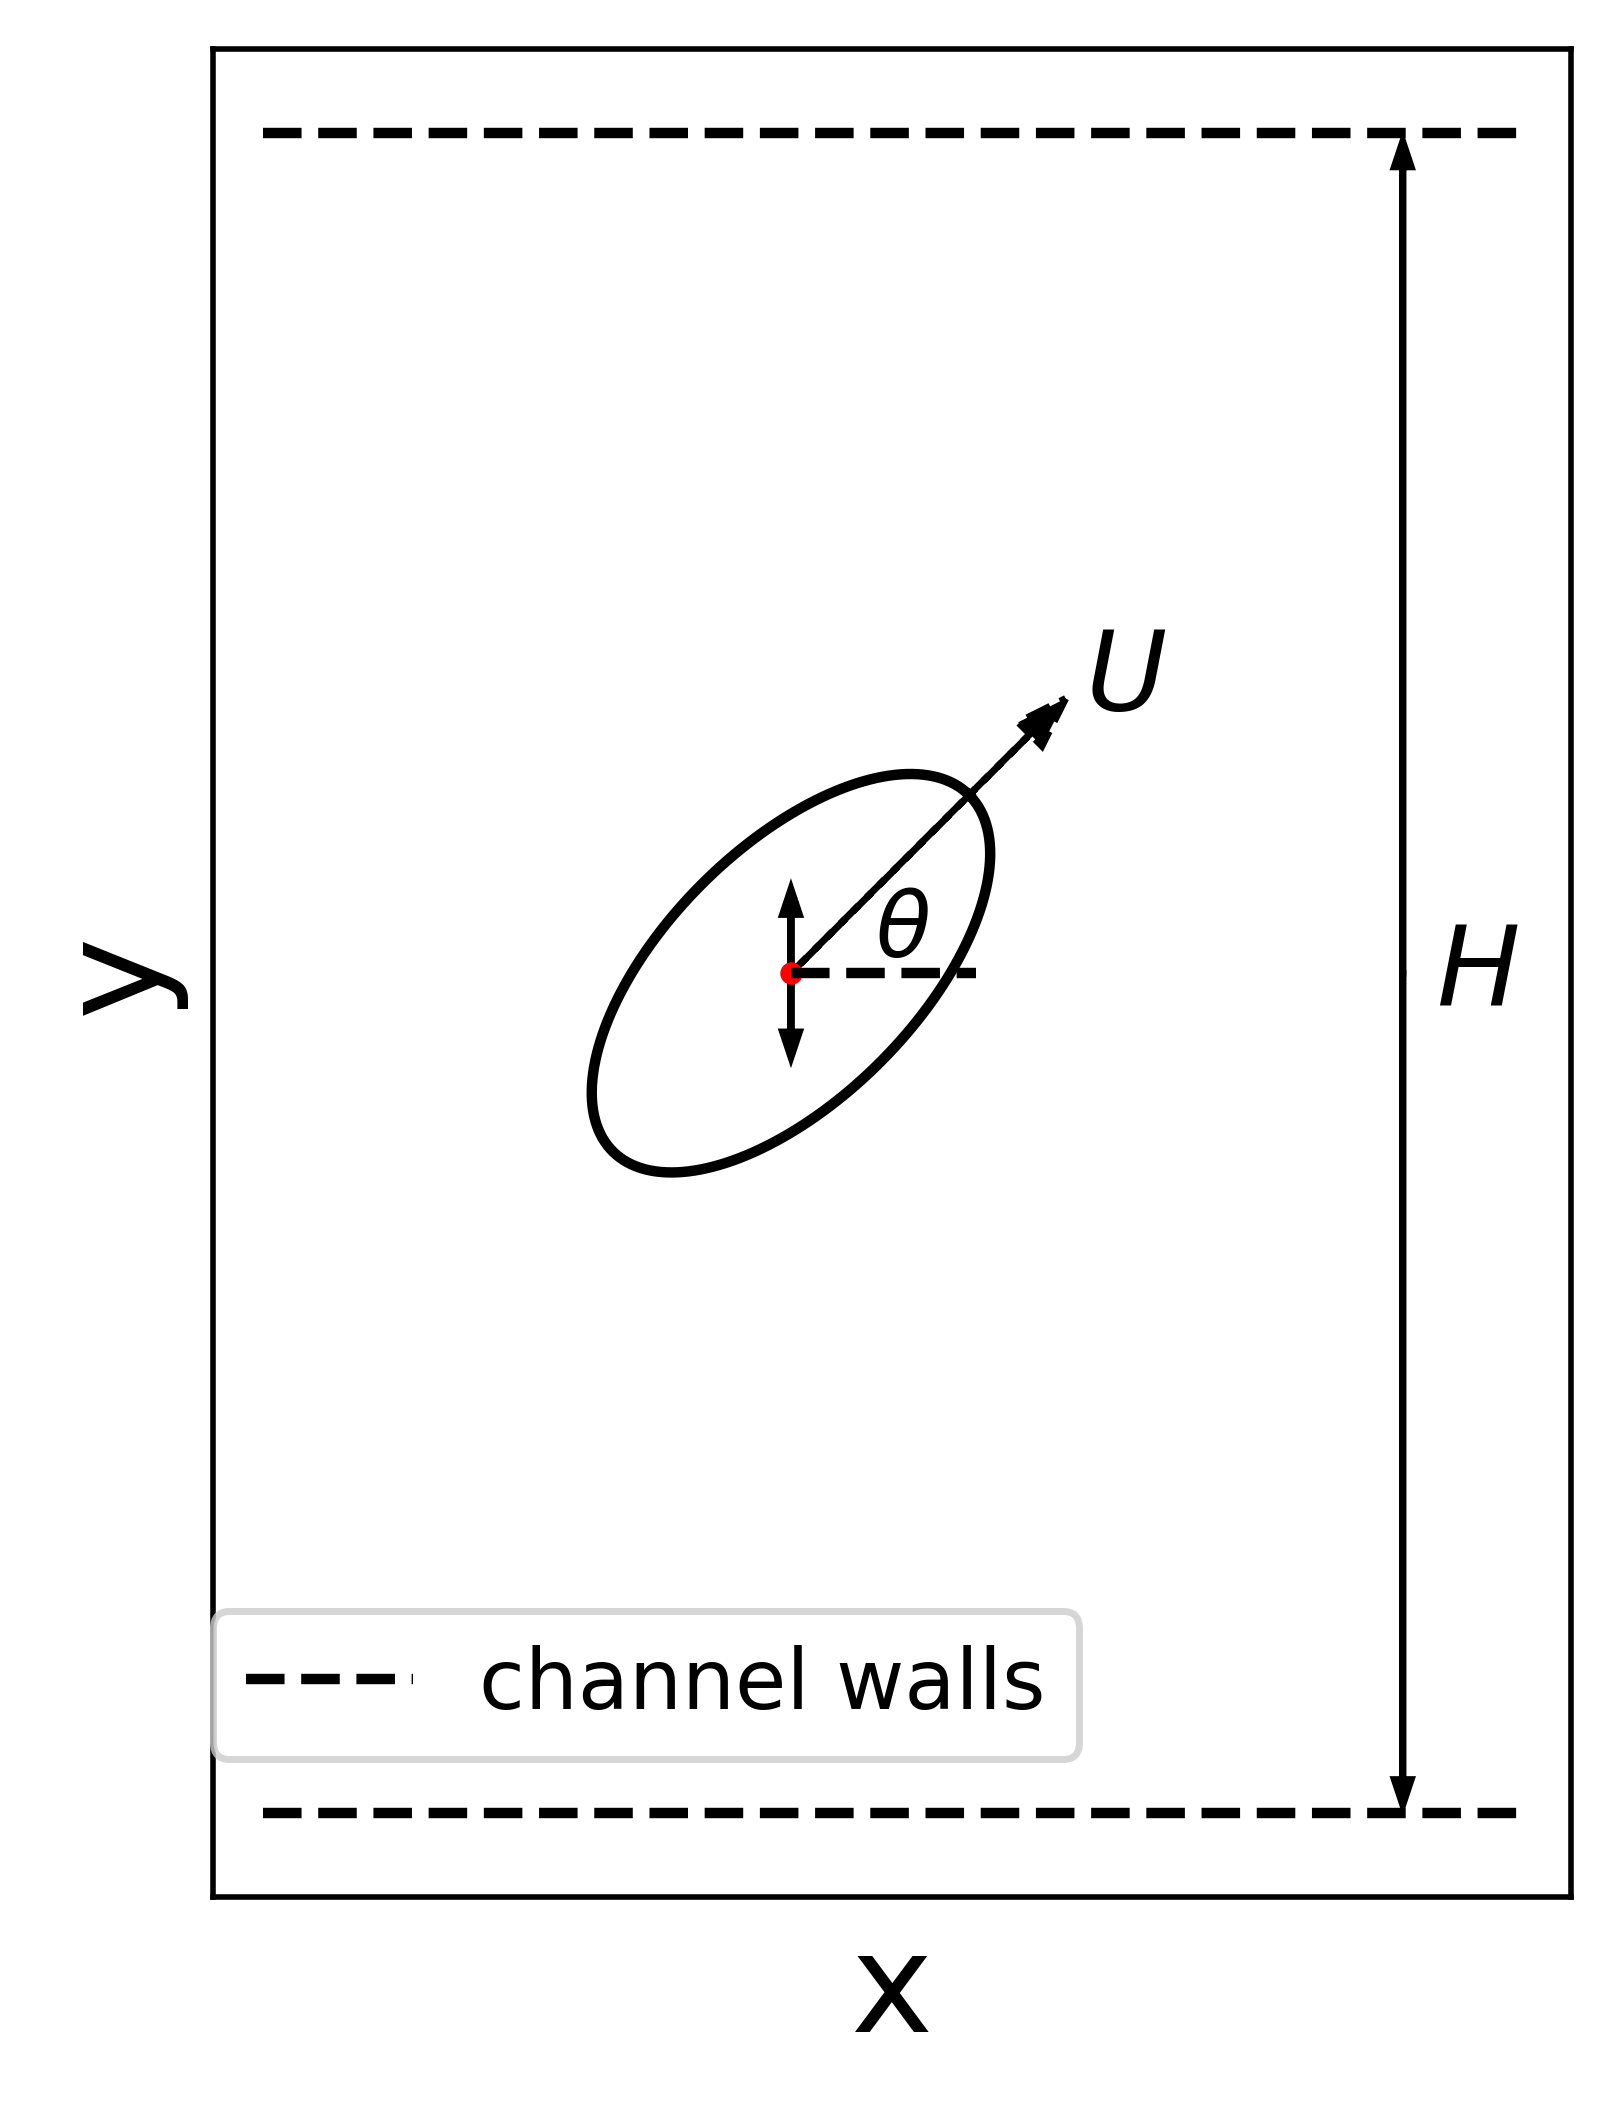
\includegraphics[scale=0.5]{graphics/model1_setup.png}
    \caption{An elliptic cell with orientation $\theta$ located within a channel of fixed height H
    and infinite width. The channel walls are considered reflective boundaries.}
    \label{fig:model1_setup}
\end{figure}

The dynamics imposed on the cell are described by the following coupled SDEs:

\begin{subequations}\label{eq:model1_sdes}
    \begin{align}
        Y(t + \Delta t) &= Y(t) + U \sin(\theta) + \sqrt{2D_y}\Delta W_1 \label{eq:model1_sdes_a} \\
        \theta(t + \Delta t) &= \theta(t) + \sqrt{2D_\theta}\Delta W_2 \label{eq:model1_sdes_b}
    \end{align}
\end{subequations}

Here, $Y(t)$ denotes the vertical position of the cell's geometric centre at time $t$,
and $\theta$ its orientation at that time. The parameters 
$D_y$ and $D_\theta$ scale the respective Brownian motion terms, modelling random
fluctuations in position and orientation. The parameter $U$ sets the deterministic speed 
of the cell's motion along the $y$-axis, thereby controlling the magnitude of the directed 
movement within the channel. We treat the upper and lower channel walls as 
reflective boundaries. Movement along the $x$-axis is disregarded, as our primary interest is in understanding
whether this system exhibits boundary accummulation behaviour. Given the channel's infinite extent along
the $x$-axis, horizontal movements have no meaningful impact on the boundary accumulation analysis. 
care primarily about whether this system exhibits boundary accummulating behaviour. With no bounds along $x$, 
it is irrelevant to consider movement along the $x$-axis. 

Our primary objective is to identify whether this system exhibits boundary accummulation behaviour. To
investigate this, we seek the stationary distribution - the long-term PDF to which the system converges as
$t \to \infty$. To obtain this stationary distribution, two approaches are available: Performing Monte Carlo 
simulations using equations \eqref{eq:model1_sdes}, or directly solving the corresponding Fokker-Planck PDE.

Both of these approaches however first require us to identify the configuration space of the system - the space of 
possible configurations of $y$ and $\theta$ the system can inhabit. As the cell's orientation $\theta$ is periodic
and thus unbounded, the vertical position $y$ is constrained by the channel walls. SPecifically, the minimum 
distance the centre of the clel can approach each channel wall depends expicitly on its orientation $\theta$. 
This dependency is illustrated in Figure \ref{fig:rolling_oval}.

\begin{figure}[htbp]
    \centering
    \includegraphics[scale=0.45]{graphics/rolling_oval.png}
    \caption{Path traced by the oval's centre, illustrating the minimum distance achievable to a horizontal
    wall as a function of orientation $\theta$}
    \label{fig:rolling_oval}
\end{figure}

The function characterising this minimum distance is termed the \textit{wall distance} function
\cite{chen2021shape}. For the specific case of an ellipse, this function is defined by:

\begin{subequations}\label{eq:wall_dist_funcs}
    \begin{align}
        y_{min}(\theta) &= \sqrt{a^2\sin^2(\theta) + b^2\cos^2(\theta)} \\
        y_{max}(\theta) &= H - \sqrt{a^2\sin^2(\theta) + b^2\cos^2(\theta)}
    \end{align}
\end{subequations}

where $a$ and $b$ are the major and minor semi-axes for the elliptic cell, respectively. 
Equations \eqref{eq:wall_dist_funcs} establish the upper and lower boundaries of the configuration space for this
system.Figure \ref{fig:configuration_space_model_1} illustrates the derived configuration space.

\begin{figure}[htbp]
    \centering
    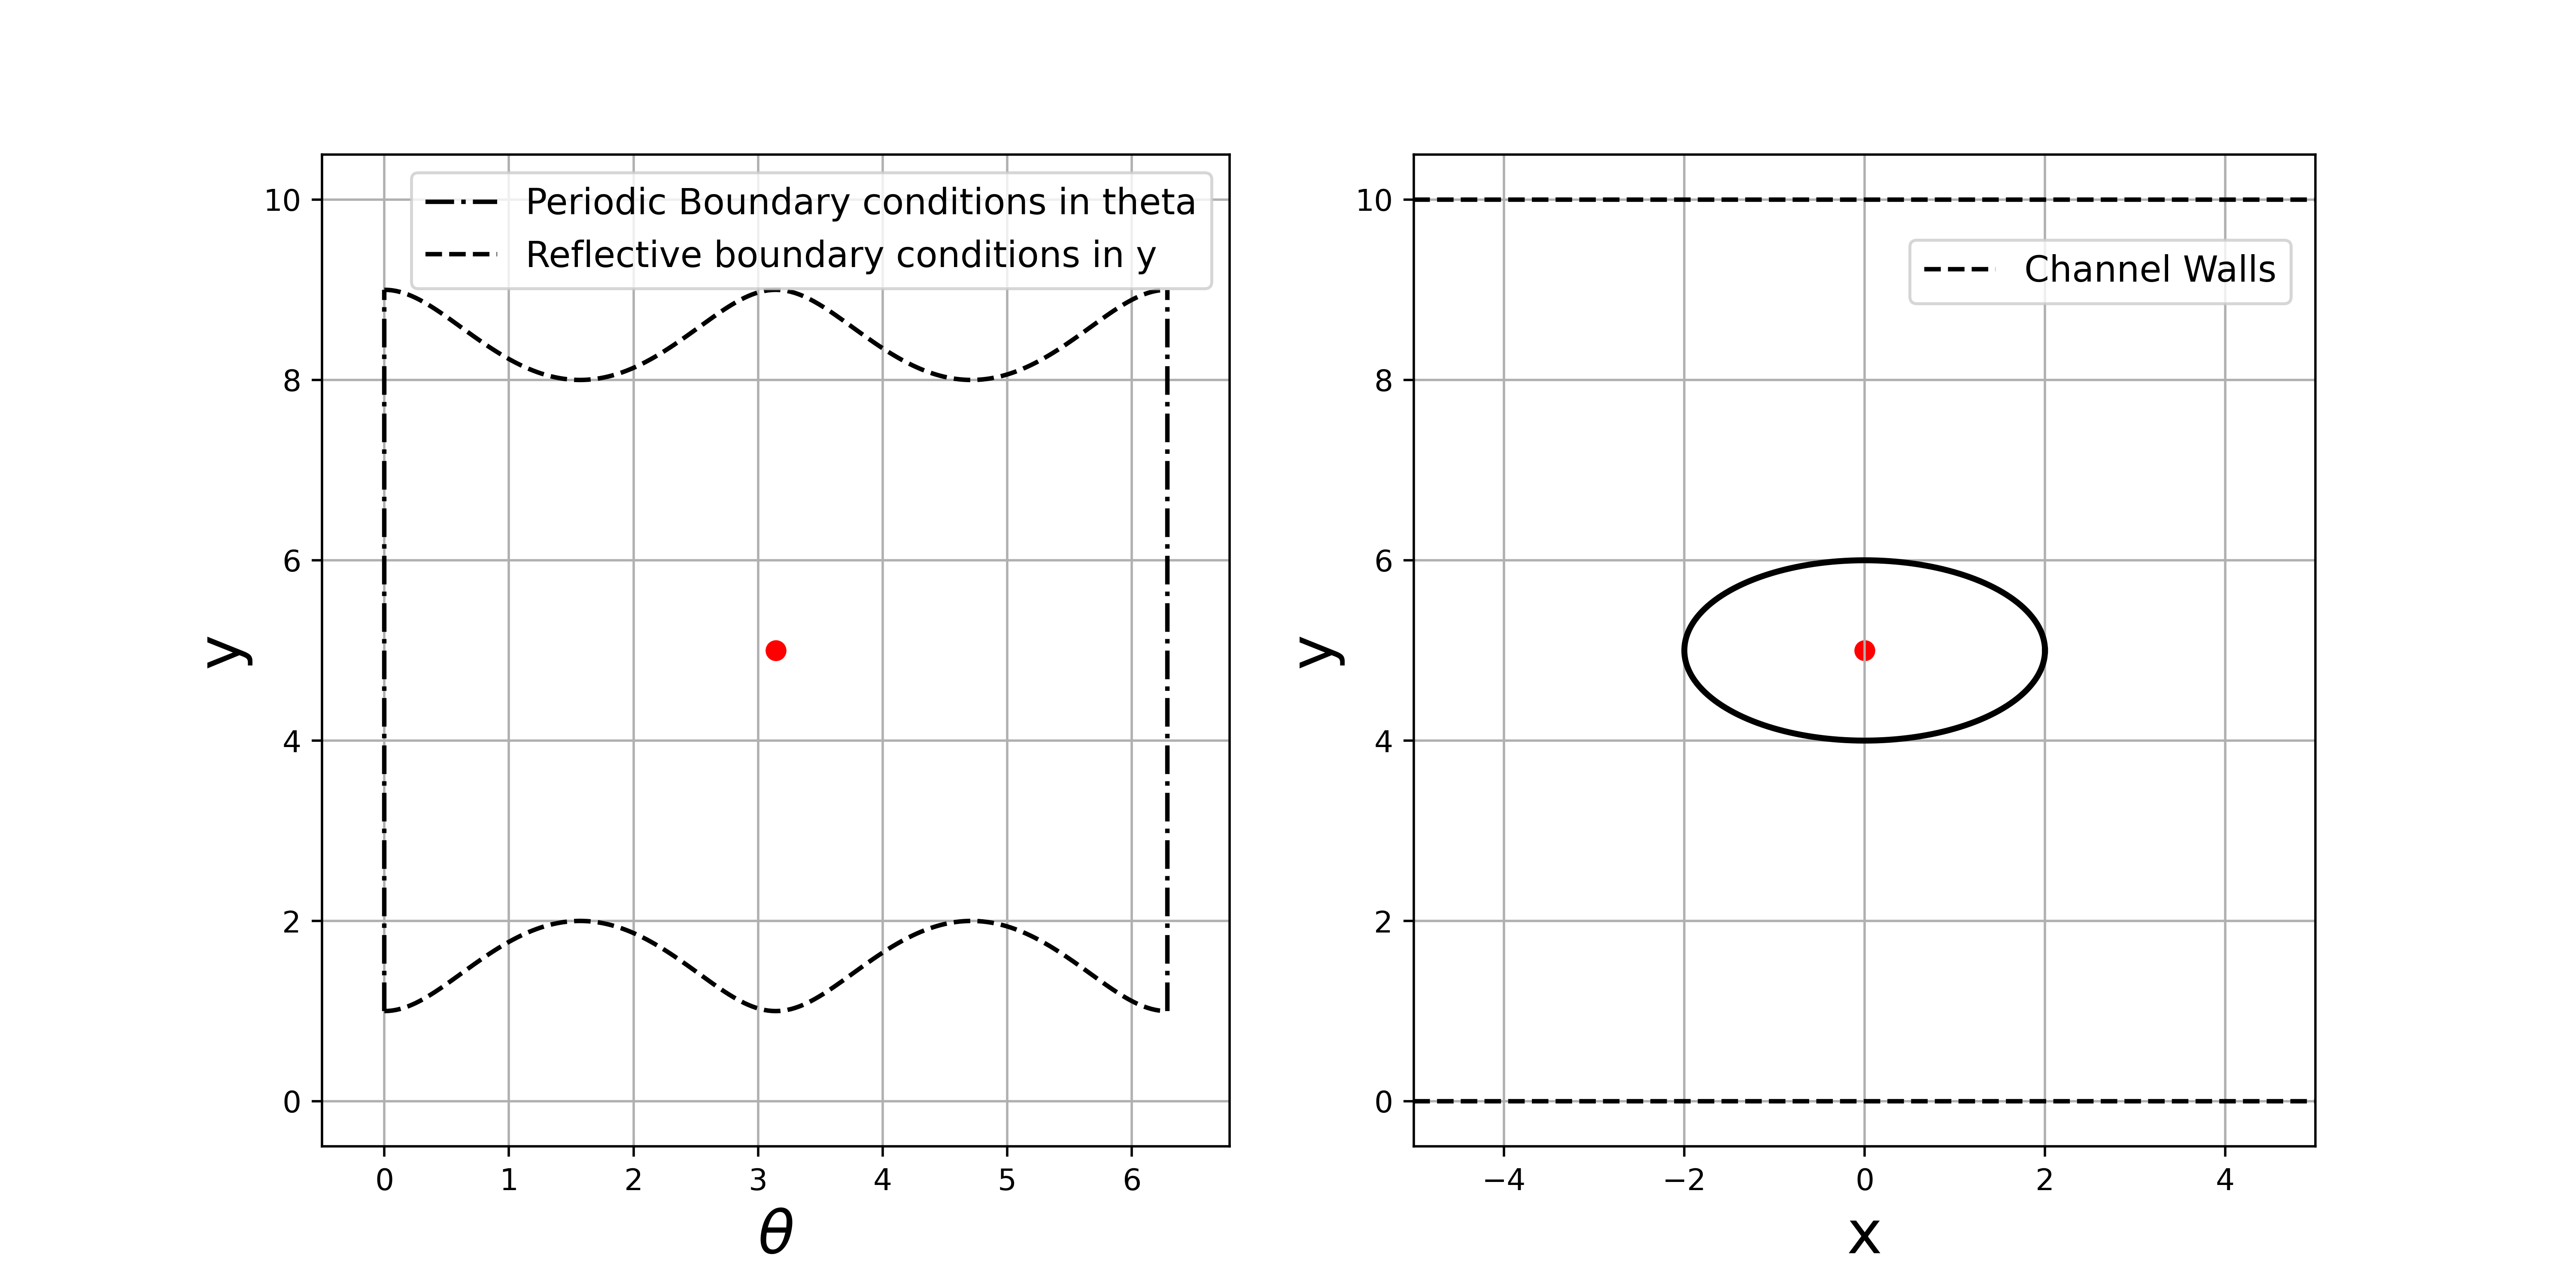
\includegraphics[scale=0.45]{graphics/config_space_1.png}
    \caption{Configuration space for Model 1 and its correspondance to 
    the physical system of a cell within a channel. Parameters used: $a=2$, $b=1$, $H=10$}
    \label{fig:configuration_space_model_1}
\end{figure}

Figure \ref{fig:configuration_space_model_1} also shows the boundary conditions 
applied to the configuration space. Periodic boundary conditions on the orientation variable
$\theta$ at $\theta=0$ and $\theta=2\pi$, while reflective boundary conditions are applied
at the upper and lower boundaries described by $y_{min}(x)$ and $y_{max}(x)$.

With a clearly bounded configuration space, the corresponding 
Fokker-Planck equation associated with equations \eqref{eq:model1_sdes} can be solved. The corresponding Fokker-Planck
equation is:

\begin{equation}\label{eq:model_1_fokker_planck}
    \frac{\partial p}{\partial t} = -\frac{\partial}{\partial y} (U\sin(\theta) p) 
    + D_{\theta} \frac{\partial^2 p}{\partial \theta^2} 
    + D_y \frac{\partial^2 p}{\partial y^2}
\end{equation}


When solving equation \eqref{eq:model_1_fokker_planck}, no-flux boundary conditions are applied at the upper and lower
boundaries along the $y$-axis, accounting for the conservation of probability within the domain. 
The finite element solver COMSOL Multiphysics\textregistered was used to numerically obtain the stationary distribution 
\cite{comsol}. The resulting PDF is presented in Figure \ref{fig:subfig_model_1_pdf}, and the resulting marginal 
distribution across the channel is displayed in Figure \ref{fig:subfig_model_1_marginal_y}.


\begin{figure}[htbp]
    \centering
    \begin{subfigure}[b]{0.45\textwidth}
        \centering
        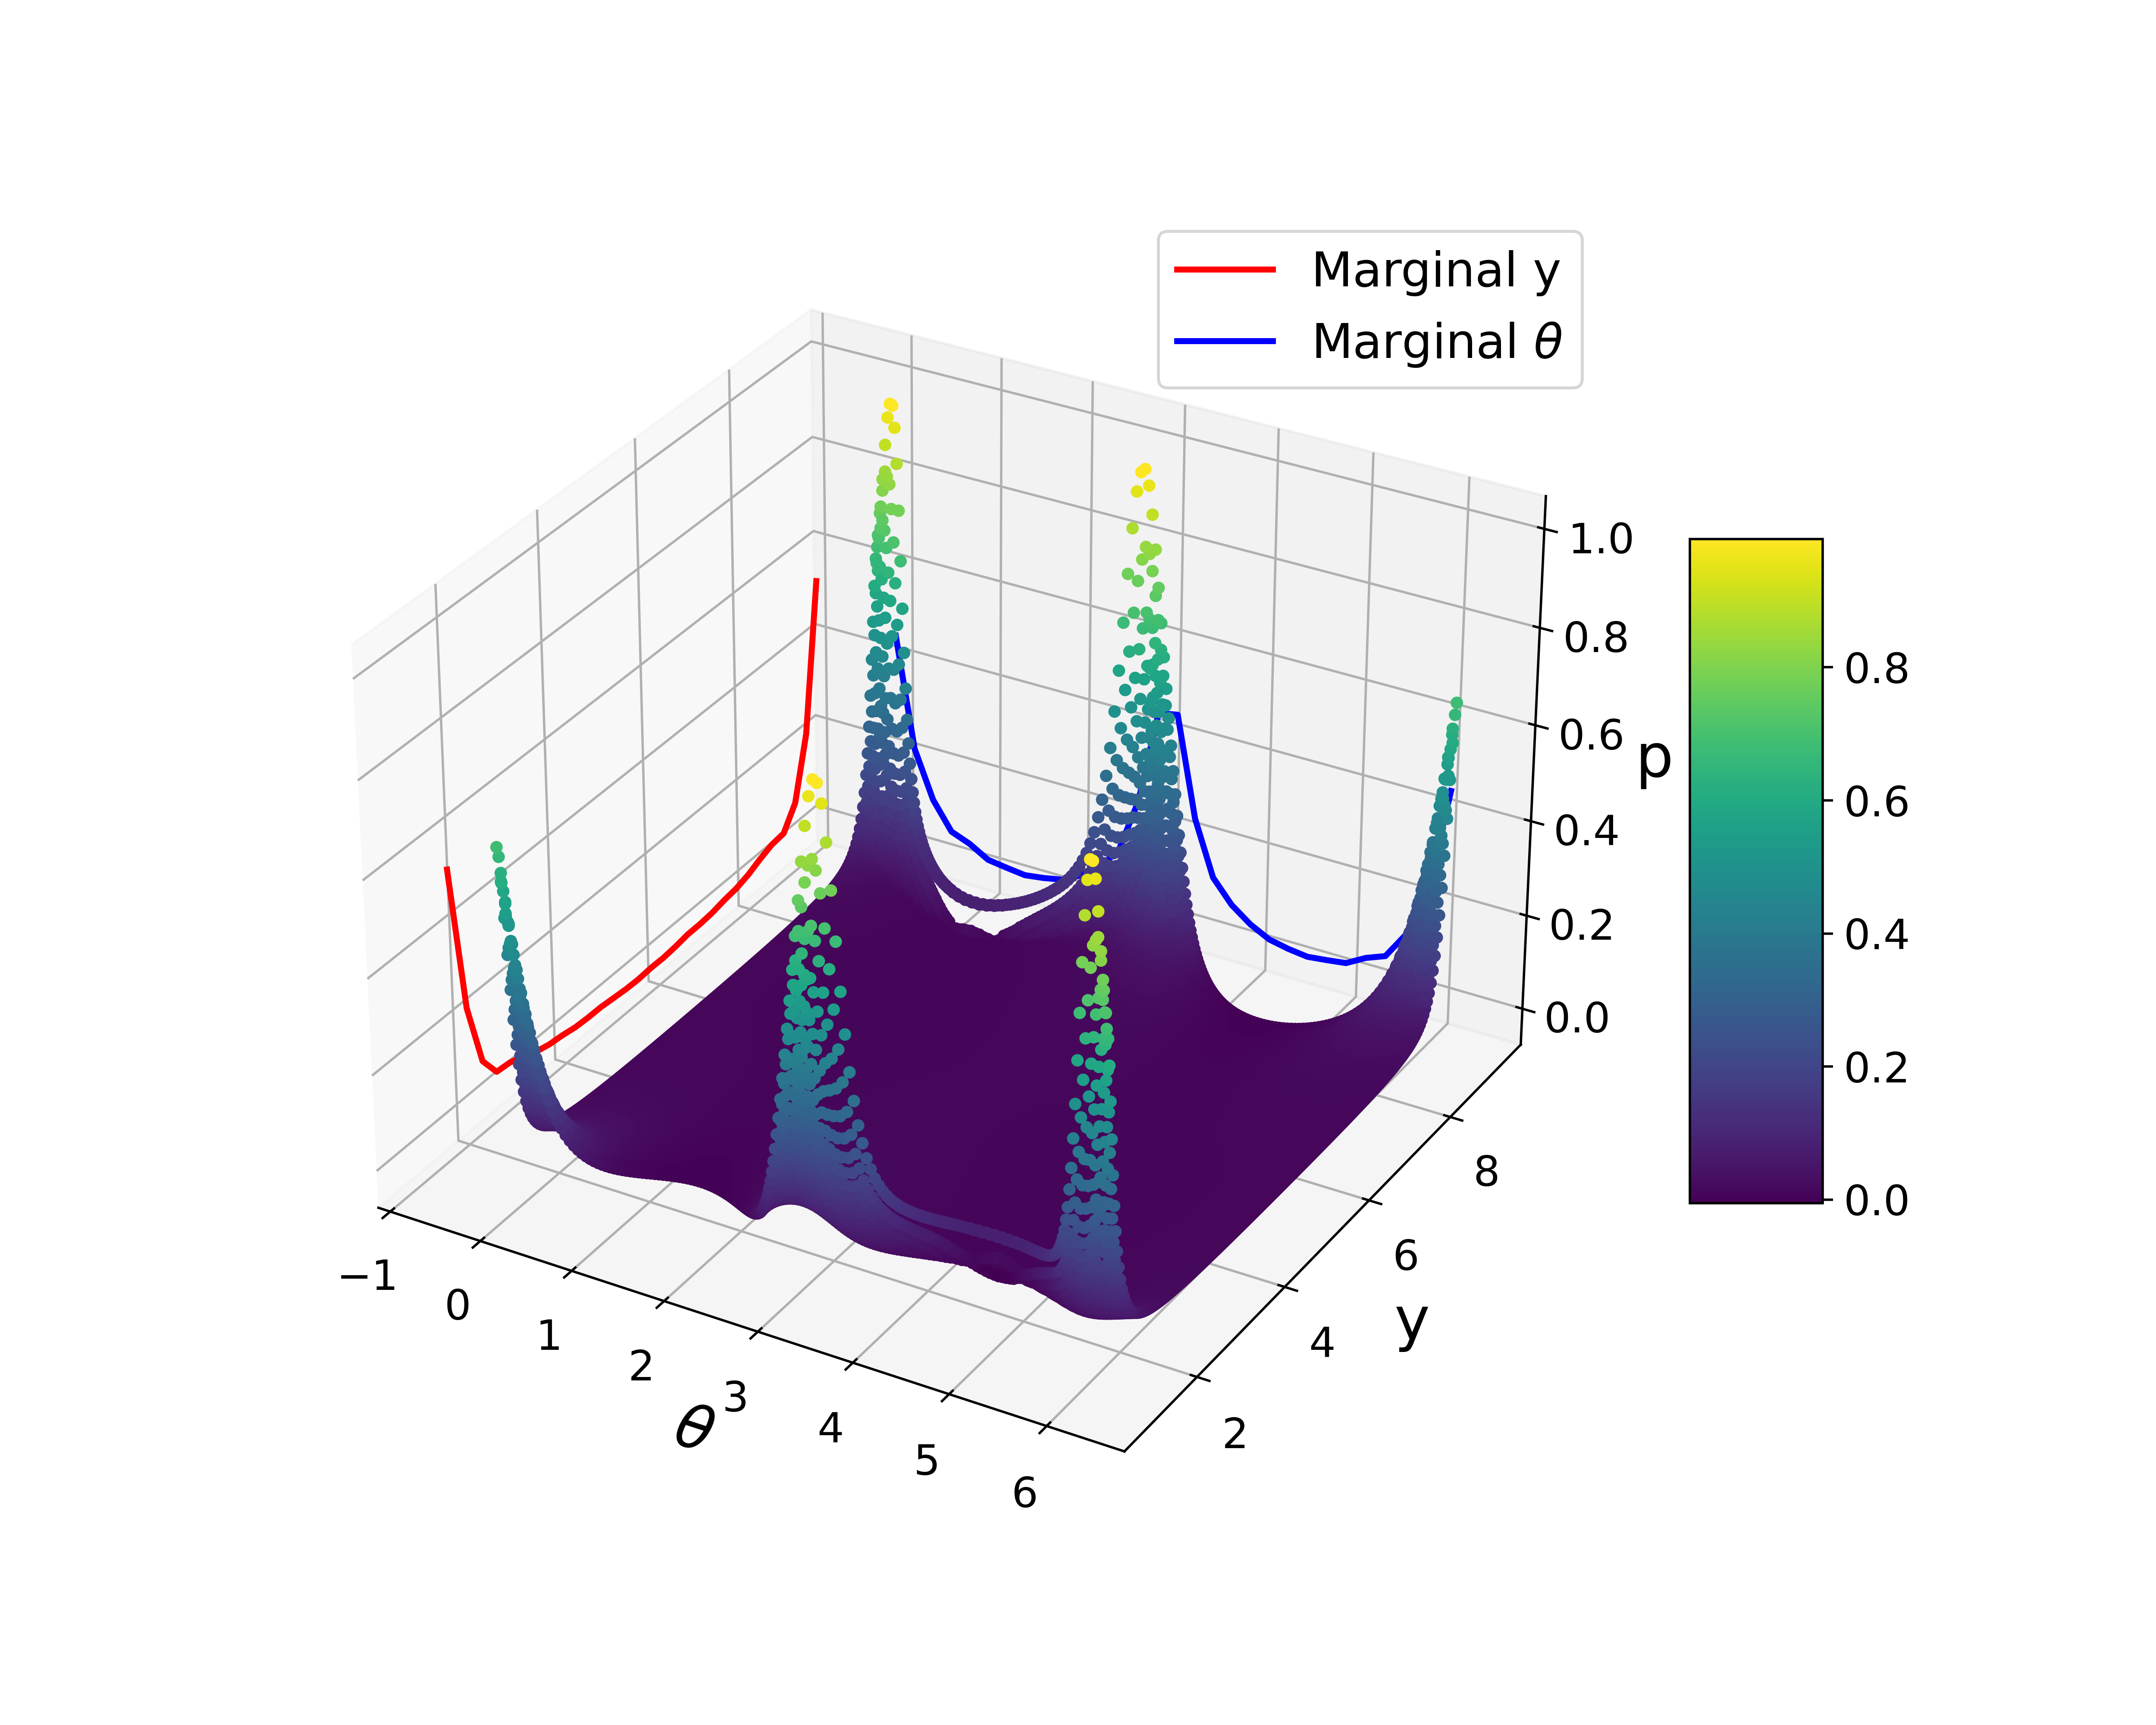
\includegraphics[width=\textwidth, trim=30 20 30 20, clip]{graphics/model_1_pdf_surface.png}
        \caption{Stationary distribution obtained for equations \eqref{eq:model1_sdes}. Marginal distributions are displayed along 
        the axes margins.}
        \label{fig:subfig_model_1_pdf}
    \end{subfigure}
    \hfill
    \begin{subfigure}[b]{0.45\textwidth}
        \centering
        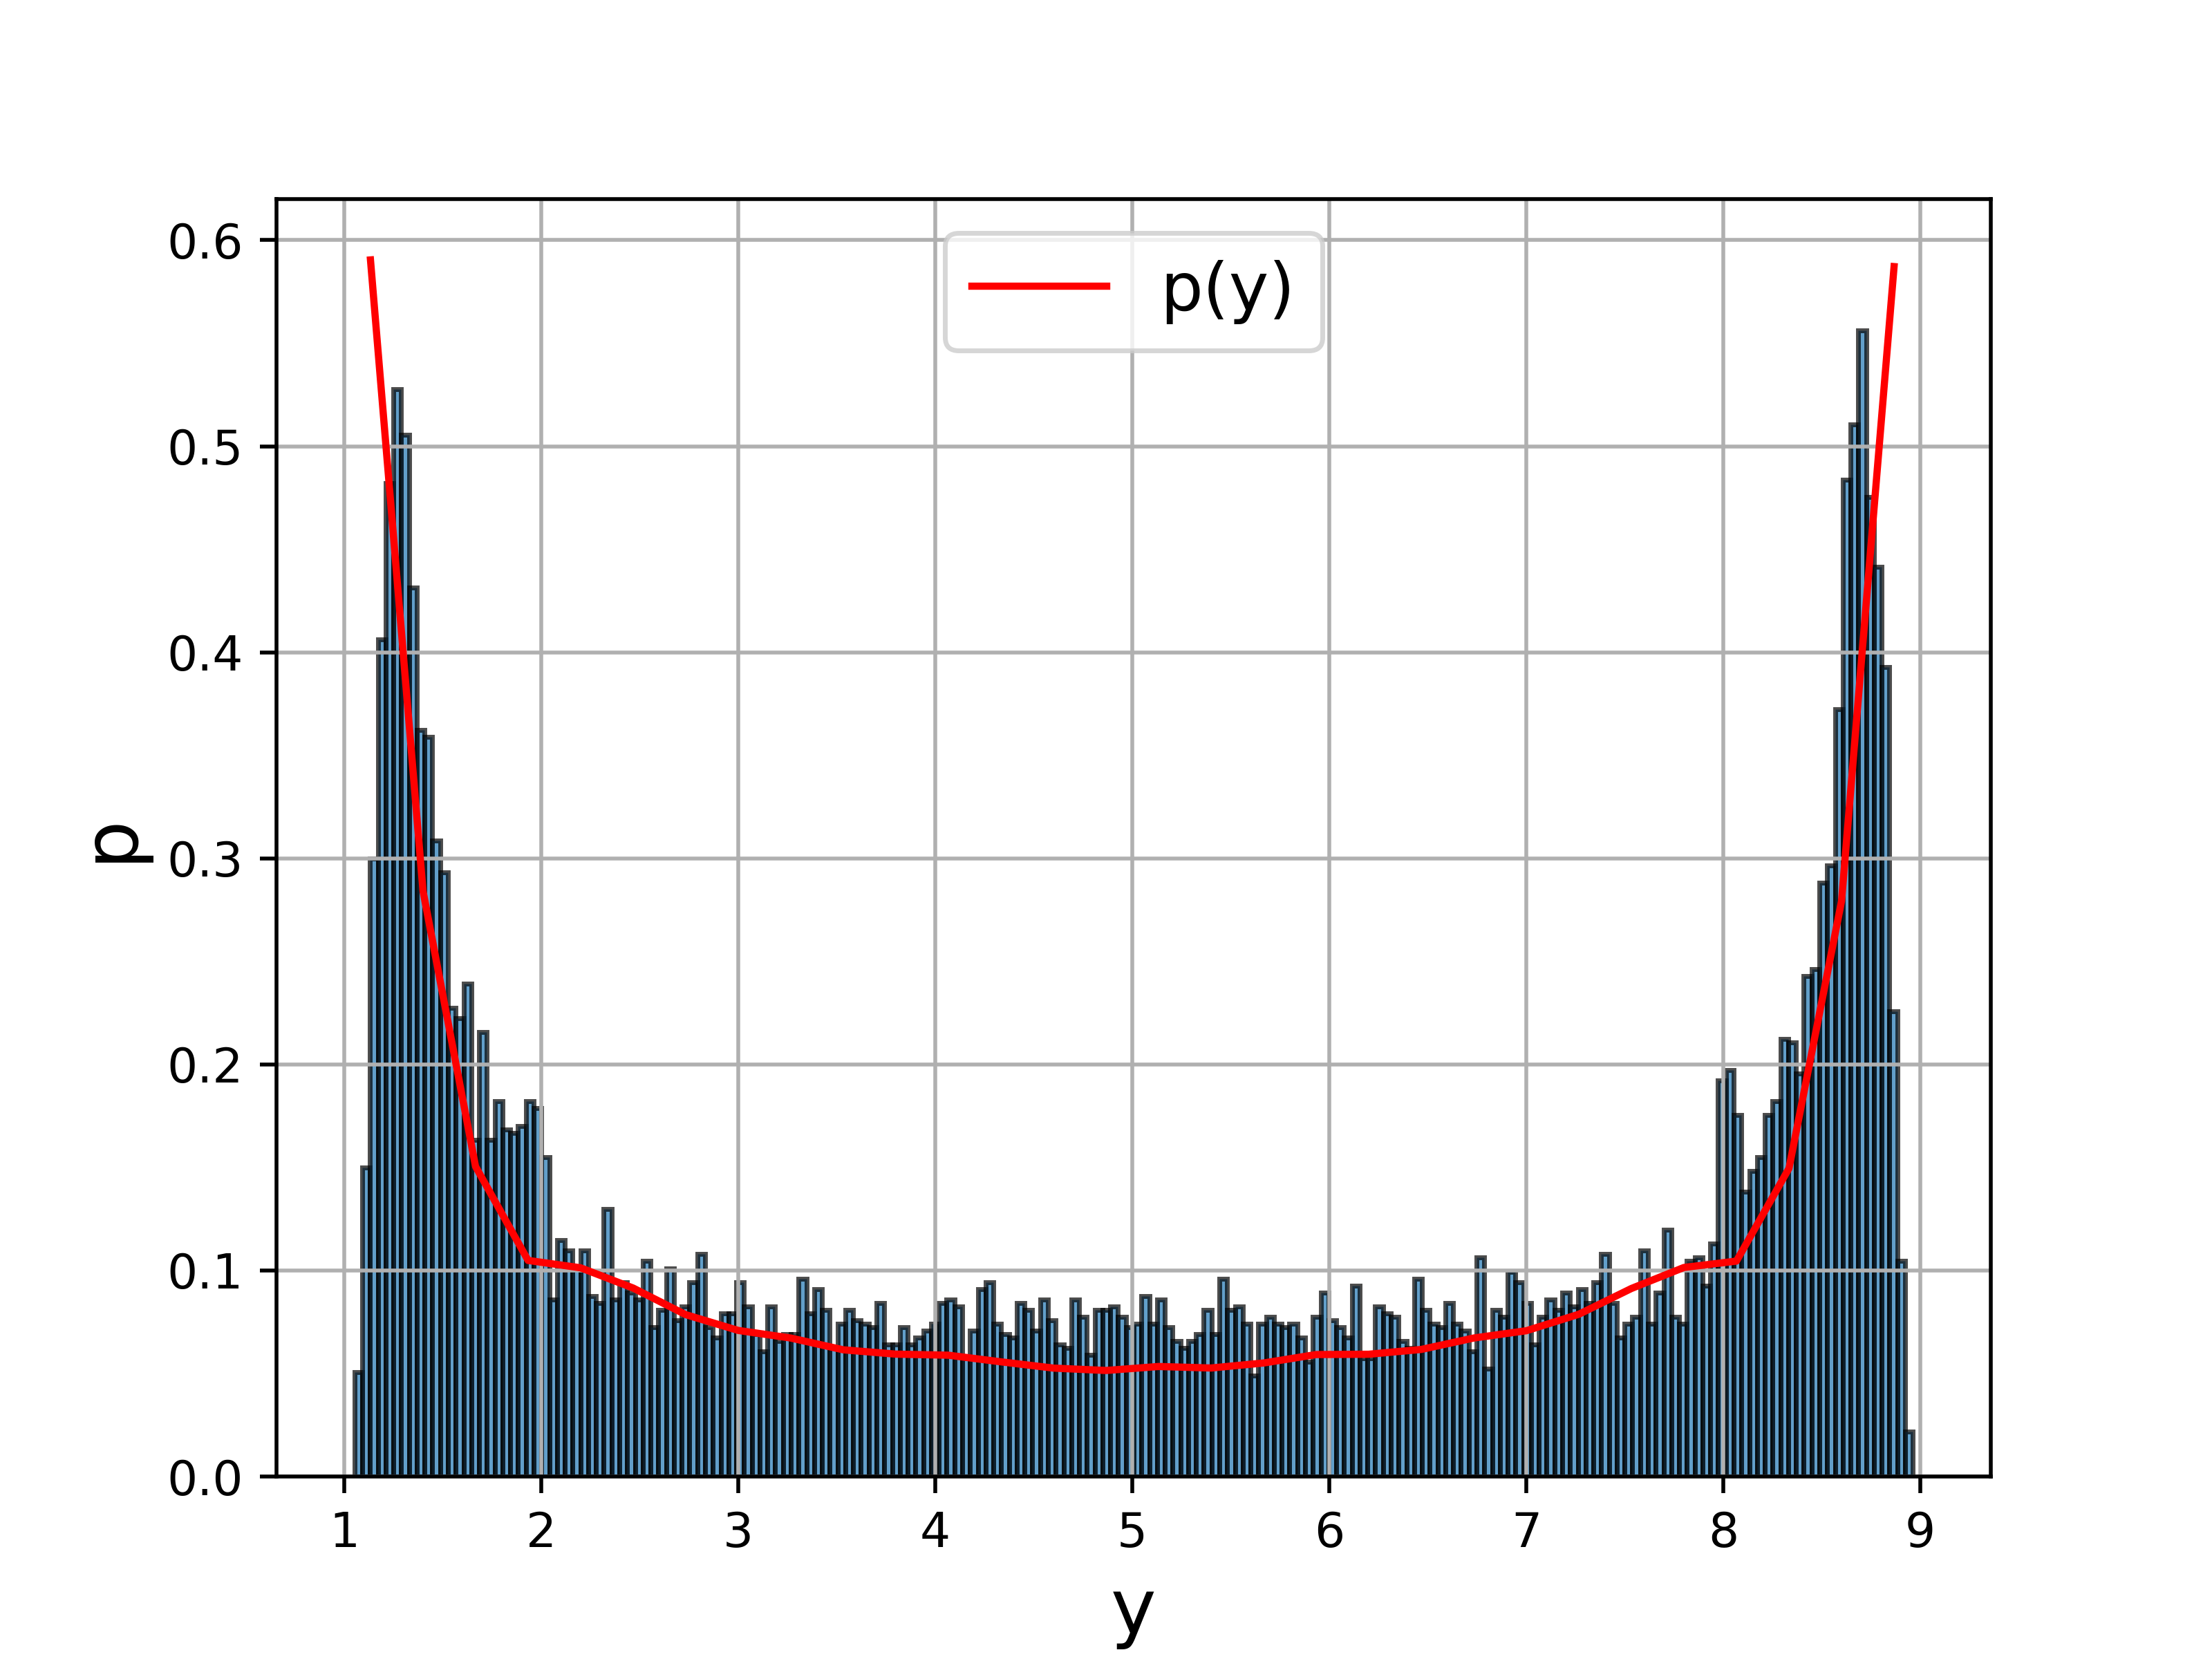
\includegraphics[width=\textwidth]{graphics/model_1_marginal_y.png}
        \caption{Marginal distributions along $y$ derived from solving the Fokker-Planck (red line) and from
         Monte Carlo simulation (histogram)}
        \label{fig:subfig_model_1_marginal_y}
    \end{subfigure}
    \caption{Comparison of stationary distribution and its marginal along $y$.}
    \label{fig:model_1_results}
\end{figure}

The marginal distribution along the $y$-axis clearly exhibits characteristic boundary accumulation behaviour. 
We attribute this phenomenon as arising from two primary mechanisms. Firstly, the drift term in equation \eqref{eq:model1_sdes_a} 
implies that, on average, the cell moves towards and eventually encounters the boundary, where it becomes constrained 
until it sufficiciently reorients. Secondly, the geometry of the configuration space contributes significantly; the elliptical
shape introduces two "hills" with reflective boundaries. These features act as barriers, hindering the ease with 
which the system can exit the boundary regions, thus enhacing the boundary accummulation.

\subsection{Model 2: Hydrodynamics Informed Model}\label{sec:hydrodynamic_model}
The second modelinvestigated was proposed by Chen \textit{et al}. \cite{chen2021shape}, 
building on the work of Spagnolie \textit{et al}. 
\cite{spagnolie2015geometric}. This advances  on the previous model by incorporating hydrodynamic interactions
with the channel walls into the SDEs for the cell.

Spagnolie \textit{et al.} approximate the velocity field around an elliptic swimmer by first treating the system as a 
\textit{stresslet} - a force dipole - and then by Faxén's Law obtaining the corresponding velocity field for a 
swimmer with elliptic shape. Figure shows two illustrative charts of a microswimmer treated as a stresslet, and the 
velocity field around this elliptic stresslet near the boundary. 

\begin{figure}[htbp]
    \centering
    \begin{subfigure}[b]{0.45\textwidth}
        \centering
        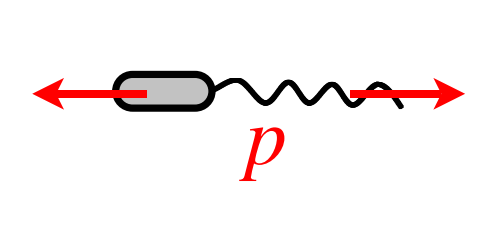
\includegraphics[width=\textwidth]{graphics/pusher_pic.png}
        \caption{Stationary}
        \label{fig:pusher_chart}
    \end{subfigure}
    \hfill
    \begin{subfigure}[b]{0.45\textwidth}
        \centering
        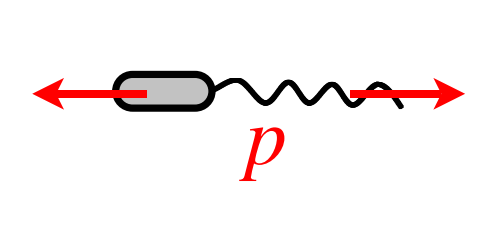
\includegraphics[width=\textwidth]{graphics/pusher_pic.png}
        \caption{Marginal}
        \label{fig:fluid_field_pusher}
    \end{subfigure}
    \caption{Comparison of stationary distribution and its marginal along $y$.}
    \label{fig:model_2_intro}
\end{figure}

% It is worth noting that in the literature microswimmers are categorised as either 
% \textit{pushers} 